\documentclass[12pt,letterpaper]{article}

% Essential packages for patent formatting
\usepackage[top=1in, bottom=1in, left=1in, right=1in]{geometry} % Proper margins
\usepackage{setspace} % For 1.5 or double line spacing
\usepackage{times} % Times Roman font (or use \usepackage{helvet} for Arial)
\usepackage{enumitem} % For customizing lists/enumerations in claims
\usepackage{fancyhdr} % For headers
\usepackage{titlesec} % For section formatting
\usepackage{graphicx} % For including drawings
\usepackage{amsmath} % For mathematical equations
\usepackage{amssymb} % For mathematical symbols
\usepackage{physics} % For quantum mechanics notation
\usepackage{braket} % For quantum state notation
\usepackage{tikz} % For drawing TikZ diagrams
\usetikzlibrary{positioning,arrows.meta}

% Set the line spacing to 1.5 (or 2.0 for double spacing)
\onehalfspacing

% Configure headers and footers
\pagestyle{fancy}
\fancyhf{} % Clear all headers and footers
\renewcommand{\headrulewidth}{0pt} % Remove header rule
\fancyfoot[C]{\thepage} % Page number at bottom center

% Configure section formatting
\titleformat{\section}
  {\normalfont\bfseries\uppercase}
  {}
  {0em}
  {}
\titlespacing{\section}{0pt}{12pt}{6pt}

% Configure subsection formatting
\titleformat{\subsection}
  {\normalfont\bfseries}
  {}
  {0em}
  {}
\titlespacing{\subsection}{0pt}{12pt}{6pt}

% Custom paragraph format with additional spacing
\setlength{\parindent}{0pt}
\setlength{\parskip}{6pt}

% Custom enumeration for claims
\newlist{patentclaims}{enumerate}{2}
\setlist[patentclaims,1]{label=\arabic*., align=left, leftmargin=2em, itemsep=1em}
\setlist[patentclaims,2]{label=\arabic*., align=left, leftmargin=2em, itemsep=0.5em}

\begin{document}

% ===== TITLE PAGE =====
\begin{center}
\Large\bfseries
SYSTEM AND METHOD FOR TEMPORAL PROCESSING USING MULTI-SHELL ARCHITECTURE WITH CONFIGURABLE COUPLING
\end{center}

\vspace{0.5in}

\vspace{1in}

\section*{CROSS-REFERENCE TO RELATED APPLICATIONS}

This application is related to co-pending U.S. Patent Application titled "SYSTEM AND METHOD FOR MULTI-PHOTON DETECTION USING QUANTUM DOT ARRAYS WITH WAVEFUNCTION-GUIDED SPECTRAL SELECTIVITY," filed concurrently herewith, the entire contents of which are hereby incorporated by reference. The temporal shell architecture described herein can be integrated with the multi-photon detection systems described in the related application to enable enhanced temporal-spectral processing capabilities.

\section*{FIELD OF THE INVENTION}

The present invention relates to temporal processing systems, and more particularly to systems and methods utilizing configurable multi-shell temporal architectures integrated with wavefunction-guided detection for enhanced temporal resolution and correlation analysis across multiple timescales. The invention encompasses both quantum and classical implementations of the temporal shell framework, with applications ranging from quantum information processing to conventional signal processing and computational systems.

\section*{BACKGROUND}

In the field of temporal information processing, conventional systems face fundamental limitations in their ability to process temporal information across multiple scales while maintaining coherence and correlation. This challenge exists in both quantum and classical domains, though with different manifestations and constraints.

In quantum systems such as quantum information processors, quantum detection and temporal processing architectures typically operate within a narrow band of temporal scales and lack the flexibility to adjust their operating parameters for different applications. Current approaches such as single-photon avalanche diodes (SPADs) and superconducting nanowire single-photon detectors (SNSPDs) are optimized for detecting individual photons but lack the ability to process temporal information in a coherent, multi-scale manner. These systems generally require photon splitting and routing to multiple detector elements when measuring multiple temporal events, resulting in reduced detection efficiency and increased system complexity.

In classical computing and signal processing domains, conventional temporal processing is typically restricted to fixed timescales determined by hardware clock rates, sampling frequencies, or filter parameters. Modern digital signal processors and neural networks can process information across different timescales, but they typically use separate processing stages with fixed parameters for each temporal domain, lacking a unified architectural framework for multi-scale temporal processing.

Moreover, both quantum and classical temporal processing architectures typically implement fixed geometric configurations that constrain their ability to model complex temporal phenomena. They are generally designed with a specific application in mind and cannot be easily reconfigured for different temporal processing tasks. This limitation becomes particularly significant when attempting to bridge microscopic phenomena with macroscopic temporal structures or when processing information that contains relevant features across widely varying timescales.

Recent theoretical advances have explored nested temporal structures, such as those described in quantum field theory, temporal logic, and hierarchical models of cognition, but practical implementations of such structures have been limited by the lack of suitable hardware architectures that can maintain coherence across multiple temporal scales. Additionally, the integration of detection principles with temporal processing remains largely unexplored, despite its potential to significantly enhance system performance.

Therefore, there remains a need for a temporal processing system that can effectively operate across multiple timescales, maintain coherence, and provide the flexibility to adapt to various applications through reconfigurable parameters and geometric configurations. Such a system would ideally leverage advanced detection principles to enhance temporal resolution and enable advanced correlation analysis in both quantum and classical implementations.

\section*{SUMMARY}

The present invention addresses the aforementioned limitations by providing a system and method for temporal processing using a configurable multi-shell architecture that integrates wavefunction-guided detection principles. In one aspect, the invention comprises a flexible temporal processing framework implementing multiple temporal shells arranged in configurable geometric patterns, a detection subsystem, and a processing system for temporal correlation analysis and state reconstruction.

The invention can be implemented in both quantum and classical domains. In quantum implementations, the temporal shells maintain quantum coherence across multiple timescales, enabling applications in quantum information processing that require intact quantum states across temporal domains. In classical implementations, the temporal shells maintain signal coherence and correlation across multiple timescales, enabling applications in advanced signal processing, pattern recognition, and computational modeling.

An advantage of the present invention is the ability to operate across multiple timescales simultaneously while maintaining coherence, whether quantum or classical depending on implementation. Additionally, the invention allows for reconfigurable shell geometries and processing parameters through electronic control systems, rather than requiring fixed architectures for each application.

The multi-shell temporal architecture of the present invention can be advantageously combined with multi-photon detection systems, such as the quantum dot array system described in the related application, to create integrated temporal-spectral processing systems with enhanced capabilities for applications ranging from quantum communication to advanced sensing and machine learning.

In various embodiments, the invention may include variable numbers of temporal shells arranged in diverse geometric configurations, different coupling schemes between shells, and application-specific optimization capabilities to enhance performance for particular use cases ranging from human perceptual processing to advanced quantum measurements.

\section*{BRIEF DESCRIPTION OF THE DRAWINGS}

FIG. 1 is a block diagram illustrating the overall system architecture of the quantum temporal processing system according to an embodiment of the present invention.

FIG. 2 is a schematic diagram depicting the configurable multi-shell temporal architecture in a hourglass configuration according to an embodiment of the present invention.

FIG. 3 is a schematic diagram showing a linear configuration of the multi-shell temporal architecture.

FIG. 4 is a schematic diagram showing a nested sphere configuration of the multi-shell temporal architecture.

FIG. 5 is a cross-sectional view of a single temporal shell structure within the multi-shell architecture.

FIG. 6 is an energy-level diagram illustrating the shell-specific processing parameters and their relationships across multiple temporal shells.

FIG. 7 is a schematic representation of wavefunction overlap between adjacent temporal shells, showing the basis for wavefunction-guided detection.

FIG. 8 is a flowchart depicting the method for quantum temporal processing using the multi-shell system.

FIG. 9 is a graph showing temporal response characteristics of the multi-shell architecture compared to conventional temporal processing systems.

FIG. 10 is a schematic diagram of the readout circuit architecture for the wavefunction-guided detection system.

\section*{DETAILED DESCRIPTION}

The following detailed description refers to the accompanying drawings which form a part of this disclosure. In the drawings, similar symbols typically identify similar components, unless context dictates otherwise. The illustrative embodiments described herein are not meant to be limiting. Other embodiments may be utilized, and other changes may be made, without departing from the spirit or scope of the subject matter presented here.

Referring first to FIG. 1, a quantum temporal processing system 100 includes a configurable multi-shell temporal architecture 101 connected to a wavefunction-guided detection subsystem 102 and a temporal correlation and state reconstruction processor 103. The multi-shell temporal architecture 101 forms the core processing element of the system and is configured with multiple temporal shells arranged in a specific geometric configuration optimized for multi-scale temporal processing.

The wavefunction-guided detection subsystem 102 is quantum-mechanically coupled to the multi-shell architecture 101 via quantum channels 104 and functions to convert quantum state information from the temporal shells into quantum signals that can be processed by the temporal correlation and state reconstruction processor 103. The processor 103 receives quantum signals from the detection subsystem 102 through quantum information channels 105 and performs temporal correlation analysis and quantum state reconstruction.

The system 100 further includes a configuration interface 106 positioned to direct control parameters into the multi-shell architecture 101, and a system controller 107 electronically connected to the multi-shell architecture 101, detection subsystem 102, and processor 103 via control lines 108. The system controller 107 functions to adjust operational parameters of the entire system, including shell frequencies, coupling strengths, detection sensitivity, and processing algorithms.

\subsection{Multi-Shell Temporal Architecture}

As shown in FIG. 2, the multi-shell temporal architecture 101 in a hourglass configuration includes multiple temporal shells 201, 202, 203, 204, 205, 206, and 207 arranged in a specific geometric pattern that resembles an hourglass. The temporal shells are positioned at precisely calculated distances from each other to optimize quantum coupling and information flow between adjacent shells.

In this exemplary embodiment, seven shells are arranged in an hourglass configuration with shells 201, 202, and 203 representing past temporal domains (distant past, intermediate past, and recent past, respectively), shell 204 representing the present moment, and shells 205, 206, and 207 representing future temporal domains (near future, intermediate future, and distant future, respectively).

Each temporal shell 201-207 has individually addressable control interfaces 208 connected to control lines 209 that extend to the system controller 107. These control interfaces 208 allow for precise tuning of the operational parameters of individual shells through application of controlled electromagnetic fields, enabling reconfigurable temporal processing of the system.

The general shell radius function that defines the geometric arrangement of the shells is given by:

$$r(i) = f(i, \{\alpha_k\})$$

where:
\begin{itemize}
    \item $f$ is a configurable function defining the geometric arrangement
    \item $\{\alpha_k\}$ is a set of configuration parameters
    \item $i$ is the shell index (1 to n, where n is the total number of shells)
\end{itemize}

For the hourglass configuration shown in FIG. 2, the radius function is defined as:

$$r(i) = r_0 \left(1 + \beta \left|\frac{i - (n+1)/2}{(n-1)/2}\right|^\gamma\right)$$

where:
\begin{itemize}
    \item $r_0$ is the minimum radius at the center (present moment)
    \item $\beta$ is an expansion coefficient
    \item $\gamma$ is a shape parameter that controls the curvature of the hourglass
    \item $n$ is the total number of shells (7 in this example)
\end{itemize}

Alternative configurations are possible, as shown in FIG. 3 (linear configuration) and FIG. 4 (nested sphere configuration). The linear configuration uses a simple radius function:

$$r(i) = r_0 + \alpha (i-1)$$

where $r_0$ is the radius of the first shell and $\alpha$ is the linear spacing between shells.

The nested sphere configuration, shown in FIG. 4, implements a three-dimensional arrangement with concentric spherical shells, where the radius function might be:

$$r(i) = r_0 \exp(\beta (i-1))$$

providing an exponential scaling of shell radii.

Referring now to FIG. 3, which shows a linear configuration of the multi-shell temporal architecture, the arrangement of temporal shells is illustrated. The linear configuration uses a simple radius function:

$$r(i) = r_0 + \alpha (i-1)$$

where $r_0$ is the radius of the first shell and $\alpha$ is the linear spacing between shells.

The arrangement of shells in the linear configuration is as follows:
\begin{itemize}
    \item TS1 (Earliest Time)
    \item TS2 (Early Time)
    \item TS3 (Present)
    \item TS4 (Later Time)
    \item TS5 (Latest Time)
\end{itemize}

The control interfaces for each shell are labeled as "Control" and are positioned to provide precise adjustment of shell parameters and are formed of materials compatible with the underlying quantum technology platform.

Referring to FIG. 5, which shows a cross-sectional view of a single temporal shell structure 201, the internal structure can be observed. The temporal shell comprises a quantum processing substrate 301 surrounded by a quantum isolation barrier 302. The quantum processing substrate 301 is selected from the group consisting of superconducting circuits, trapped ion arrays, quantum dot arrays, nitrogen-vacancy diamond structures, or other suitable quantum processing materials that provide the desired quantum information processing properties. The isolation barrier 302 is selected to have appropriate quantum coherence protection properties, and may consist of electromagnetic shielding, photonic bandgap materials, or other suitable materials that provide sufficient isolation for maintaining quantum states.

The temporal shell structure 201 further includes quantum coupling elements 303 that enable controlled quantum information exchange with adjacent shells. These coupling elements are implemented using entangled photon channels, superconducting transmission lines, or other quantum-coherent coupling mechanisms. Control interfaces 208 are positioned to provide precise adjustment of shell parameters and are formed of materials compatible with the underlying quantum technology platform.

\subsection{Shell-Specific Processing Parameters}

FIG. 6 illustrates the shell-specific processing parameters for each temporal shell. Each shell (represented as TS1 401, TS2 402, through TSn 403) is engineered to have specific operational parameters. The base frequency parameter is represented as $\omega_i$ (411, 421, 431), while the decay rate parameters are labeled as $\gamma_i$ (412, 422, 432), and the coupling coefficients as $\kappa_{ij}$ (413, 423, 433).

For the seven-shell hourglass configuration shown in FIG. 2, exemplary parameters are:

\begin{itemize}
    \item Distant Past (Shell 201): $\omega_1 = 0.7\omega_0$, $\gamma_1 = 0.2\gamma_0$
    \item Intermediate Past (Shell 202): $\omega_2 = 0.85\omega_0$, $\gamma_2 = 0.3\gamma_0$
    \item Recent Past (Shell 203): $\omega_3 = 0.95\omega_0$, $\gamma_3 = 0.4\gamma_0$
    \item Present (Shell 204): $\omega_4 = 1.0\omega_0$, $\gamma_4 = 0.5\gamma_0$
    \item Near Future (Shell 205): $\omega_5 = 0.95\omega_0$, $\gamma_5 = 0.4\gamma_0$
    \item Intermediate Future (Shell 206): $\omega_6 = 0.85\omega_0$, $\gamma_6 = 0.3\gamma_0$
    \item Distant Future (Shell 207): $\omega_7 = 0.7\omega_0$, $\gamma_7 = 0.2\gamma_0$
\end{itemize}

where $\omega_0$ and $\gamma_0$ are reference frequency and decay rate values that can be adjusted based on the specific application requirements.

The shell frequencies exhibit symmetry around the present moment (Shell 204), with decreasing frequencies as one moves toward either the distant past or distant future. This frequency profile enables the system to process temporal information at different rates appropriate to the temporal distance from the present.

The mathematical framework that describes the dynamics of each temporal shell can be expressed through quantum mechanical operators. The state of shell $i$ can be represented as:

$$|\Psi_i\rangle = \sum_j \alpha_{i,j} |j_i\rangle$$

where $|j_i\rangle$ represents the $j$-th basis state of the $i$-th shell, and $\alpha_{i,j}$ are complex probability amplitudes.

The Hamiltonian governing the dynamics of each individual shell is:

$$H_i = \hbar\omega_i \sum_j j a_j^{(i)\dagger} a_j^{(i)} - i\hbar\gamma_i \sum_j (a_j^{(i)\dagger} a_j^{(i)})^2$$

where $a_j^{(i)\dagger}$ and $a_j^{(i)}$ are creation and annihilation operators for the $j$-th mode of the $i$-th shell.

\subsection{Inter-Shell Coupling Framework}

The coupling between temporal shells is critical for the operation of the system and is described by the interaction Hamiltonian:

$$H_{\text{coupling},i,j} = \sum_{k,l} \kappa_{kl}^{(i,j)} (a_k^{(i)\dagger} a_l^{(j)} + a_k^{(i)} a_l^{(j)\dagger})$$

where $\kappa_{kl}^{(i,j)}$ are the coupling coefficients between mode $k$ of shell $i$ and mode $l$ of shell $j$.

The coupling strength typically follows a profile that depends on the geometric configuration. For the hourglass configuration, adjacent shell coupling is strongest at the narrow waist (near the present moment) and decreases toward the wider regions (distant past and future). The coupling profile is designed to facilitate efficient information flow between adjacent temporal domains while maintaining appropriate isolation between distant domains.

Referring to FIG. 7, the quantum wavefunction overlap between adjacent temporal shells in the architecture is illustrated. The quantum wavefunctions in temporal shells TS1 501 and TS2 502 are represented by $\psi_1(\vec{r})$ 511 and $\psi_2(\vec{r})$ 512, respectively. When the temporal shells are positioned at an optimal separation distance $d$ 520, their wavefunctions exhibit a controlled overlap in the region 530. This overlap region is critical for the wavefunction-guided detection mechanism of the invention.

The degree of wavefunction overlap can be quantified by the overlap integral:

$$S_{12} = \int \psi_1^*(\vec{r})\psi_2(\vec{r})d\vec{r}$$

The value of $S_{12}$ determines the strength of quantum mechanical coupling between the shells and can be precisely controlled through the geometric arrangement of the multi-shell architecture and the applied control parameters. This controlled coupling enables the formation of collective temporal modes that span multiple shells, providing the basis for the detection of correlated temporal events across different timescales.

\subsection{Wavefunction-Guided Detection Subsystem}

The wavefunction-guided detection subsystem 102 implements a quantum detection framework based on the photon wavefunction principles. The system projects incoming temporal information onto the multi-shell architecture basis states through the operator:

$$\hat{D}(x,t) = \sum_j \int dx' \chi_j(x-x')\Psi_{\text{photon}}^\dagger(x')\Phi_{\text{QD},j}(x)$$

where:
\begin{itemize}
    \item $\hat{D}(x,t)$ is the detection operator at position $x$ and time $t$
    \item $\chi_j(x-x')$ is a coupling function between the photon field and the $j$-th quantum dot
    \item $\Psi_{\text{photon}}^\dagger(x')$ is the photon creation operator at position $x'$
    \item $\Phi_{\text{QD},j}(x)$ is the quantum dot state function for the $j$-th quantum dot
\end{itemize}

The photon wavefunction evolves according to the equation:

$$i\hbar \frac{\partial}{\partial t}\Psi_{\text{photon}}(x,t) = (H + T^{(t)})\Psi_{\text{photon}}(x,t)$$

where $H$ is the free photon Hamiltonian and $T^{(t)}$ is an operator that ensures the wavefunction remains within the physically allowed subspace of transverse, gauge-invariant states during time evolution.

For multi-photon states, the system implements a tensor product structure:

$$\Psi_{\text{total}} = \sum_{i_1,...,i_N} c_{i_1,...,i_N}\bigotimes_{k=1}^N \Psi_{i_k}(x_k,t_k)$$

where $c_{i_1,...,i_N}$ are complex coefficients specifying how the single-photon wavefunctions combine to form the full multi-photon state.

The probability of detecting a specific temporal pattern across multiple shells is given by:

$$P(x_1,...,x_N;t) = |\langle \text{vac}|\hat{D}(x_1,t)...\hat{D}(x_N,t)|\Psi_{\text{total}}\rangle|^2$$

This framework allows the system to detect correlated temporal events across different shells while maintaining quantum coherence throughout the process.

\subsection{System Operation}

In operation, the quantum temporal processing system 100 functions as follows, as depicted in the flowchart of FIG. 8. First, at step 601, the system is initialized by configuring the multi-shell temporal architecture through application of appropriate control parameters. This involves establishing the desired geometric configuration, shell frequencies, decay rates, and coupling coefficients for the specific application.

Next, at step 602, temporal information is directed onto the multi-shell architecture through quantum information channels. When temporal events interact with the multi-shell architecture at step 603, they induce transitions between quantum states in one or more temporal shells, creating a specific excitation pattern across the architecture.

This excitation pattern is then measured by the wavefunction-guided detection subsystem at step 604, which converts the quantum state information into signals that can be processed. The signals are processed by the temporal correlation and state reconstruction processor at step 605, which performs temporal correlation analysis to identify relationships between events across different timescales.

At step 606, the original temporal quantum state is reconstructed based on the measured excitation pattern and temporal correlations. Finally, at step 607, the reconstructed temporal information is output for use in quantum information processing, temporal analysis, or other applications.

The temporal response characteristics of the multi-shell architecture compared to conventional temporal processing systems are illustrated in FIG. 9. The graph shows the temporal resolution 701 as a function of timescale for the multi-shell architecture system 702 compared to a conventional processor with fixed timescale sensitivity 703. The multi-shell architecture exhibits enhanced resolution peaks 704, 705, and 706 at multiple timescales simultaneously, with significantly reduced interference between temporal channels compared to the narrower response curve 707 of conventional systems.

Referring to FIG. 10, the readout circuit architecture for the wavefunction-guided detection subsystem 102 is shown in detail. The readout circuit includes quantum-limited amplifiers 801 connected to each temporal shell in the architecture through quantum channels 802. The amplifiers 801 feed into quantum state analyzers 803, which process the quantum signals for state reconstruction. A quantum timing control unit 804 ensures precise synchronization of the readout process across all temporal shells, which is critical for temporal correlation analysis.

The readout circuit further includes a quantum multiplexer 805 that combines the quantum signals from multiple analyzers and transmits them to the temporal correlation and state reconstruction processor 103 through a quantum information interface 806. The entire readout circuit is controlled by a local quantum controller 807 that receives commands from the main system controller 107 through the control interface 808.

\subsection{Classical Implementations of the Multi-Shell Architecture}

While the previous sections have focused primarily on quantum implementations of the multi-shell temporal architecture, the fundamental principles can be effectively translated into classical implementations with significant advantages over conventional temporal processing systems.

In classical implementations, the temporal shells can be realized as specialized processing units with configurable parameters and interconnections. Each shell represents a processing domain optimized for a specific timescale, with the shell's parameters (analogous to $\omega_i$ and $\gamma_i$ in quantum implementations) determining its temporal response characteristics. The coupling between shells (analogous to $\kappa_{ij}$ in quantum implementations) is implemented through signal pathways with configurable weights and delays.

Classical implementations can utilize various hardware platforms, including:

\begin{itemize}
    \item Digital signal processors with configurable filter banks and interconnections
    \item Field-programmable gate arrays (FPGAs) with reconfigurable processing elements
    \item Application-specific integrated circuits (ASICs) with hardwired shell structures optimized for specific applications
    \item Neuromorphic computing platforms with time-constant tunable elements
    \item Mixed-signal circuits combining analog temporal processing with digital control
\end{itemize}

The mathematical framework for classical implementations maintains structural similarities to the quantum framework but replaces quantum operators with classical signal processing operations. For example, the state of shell $i$ can be represented as a continuous or discrete signal $s_i(t)$ evolving according to shell-specific equations such as:

$$\frac{d s_i(t)}{dt} = -\gamma_i s_i(t) + \omega_i \mathcal{F}[s_i(t)] + \sum_j \kappa_{ij} s_j(t)$$

where $\mathcal{F}$ represents a nonlinear transformation function that can be tailored to the specific application.

The coupling between classical shells follows principles similar to those of resonance and entrainment in coupled oscillator systems, but with enhanced flexibility due to the configurable nature of the coupling parameters. This enables the formation of complex temporal processing hierarchies that can detect and analyze patterns across multiple timescales.

An advantage of classical implementations is the potential for higher operating temperatures, reduced system complexity, and easier integration with existing electronic systems. The classical multi-shell temporal architecture can be especially valuable in applications such as:

\begin{itemize}
    \item Multi-scale time series analysis for financial or environmental data
    \item Hierarchical pattern recognition in temporal signals
    \item Adaptive filtering with simultaneous operation across multiple frequency bands
    \item Biosignal processing for medical applications
    \item Speech and audio processing with natural timescale hierarchies
\end{itemize}

The classical implementation can also serve as a transitional technology, allowing systems to leverage the multi-shell architectural principles while quantum implementations continue to mature. This creates a natural technology progression path from classical to quantum temporal processing as quantum hardware capabilities advance.

\subsection{Integration with Multi-Photon Detection Systems}

The temporal processing framework described in this invention can be advantageously integrated with advanced photon detection systems, particularly those utilizing quantum dot arrays with wavefunction-guided spectral selectivity as described in the related application.

This integration creates a comprehensive temporal-spectral processing system with enhanced capabilities for quantum information processing and sensing applications. The quantum dot array provides high-fidelity multi-photon detection with spectral discrimination, while the temporal shell architecture adds multi-scale temporal processing capabilities.

The integration can be implemented through various approaches:

\begin{itemize}
    \item Direct coupling: Quantum dot excitation patterns feed directly into the temporal shell architecture
    \item Shared quantum registers: Quantum information is exchanged between the detection system and temporal processor
    \item Hybrid architecture: Classical temporal shells process information from quantum photon detectors
    \item Cascaded system: Temporal processing follows spectral analysis in a sequential pipeline
\end{itemize}

The combined system enables advanced applications such as:

\begin{itemize}
    \item Quantum communication with enhanced temporal-spectral coding
    \item Quantum sensing with multi-dimensional discrimination capabilities
    \item Quantum-enhanced machine learning with rich feature extraction
    \item Advanced spectroscopy with temporal correlation analysis
\end{itemize}

This integration represents a powerful approach to addressing complex sensing and information processing challenges that require both spectral and temporal analysis across multiple scales.

\subsection{Specific Implementations}

\subsubsection{Seven-Shell Hourglass Configuration}

A specific implementation of the system optimized for human perceptual timescales features the seven-shell hourglass configuration described earlier. This configuration is particularly suited for applications involving human-machine interfaces, cognitive processing simulations, and perceptual analysis systems.

In this implementation, the base frequency, decay rate, and coupling coefficients are optimized to match characteristic human temporal perception ranges, which span from milliseconds to minutes. The hourglass geometry provides stronger coupling near the present moment (shell 204) and progressively weaker coupling toward the distant past and future shells, mirroring human perception's focus on the present with diminishing resolution toward temporal extremes.

\subsubsection{Linear Configuration}

A simplified implementation for quantum optics applications features a linear arrangement of temporal shells, as shown in FIG. 3. This configuration is suited for applications requiring uniform temporal resolution across a specific range of timescales, such as quantum communication protocols and certain quantum sensing applications.

In the linear configuration, coupling strengths between adjacent shells can be uniform or follow a predefined gradient, depending on the specific application requirements. This implementation is typically used with a smaller number of shells (3-5) and emphasizes computational efficiency and implementation simplicity over the more complex geometric arrangements.

\subsubsection{Nested Sphere Configuration}

A three-dimensional implementation features concentric spherical shells, as shown in FIG. 4. This configuration enables full three-dimensional coupling between temporal shells, allowing for more complex temporal correlation analysis and enhanced directional sensitivity.

The nested sphere configuration is particularly suited for applications involving spatiotemporal analysis, quantum imaging with temporal resolution, and advanced quantum simulation tasks. The three-dimensional arrangement allows for angular resolution in temporal processing, enabling the system to detect and analyze directional temporal patterns that would be difficult to identify with simpler configurations.

\subsection{Methods of Manufacture}

Methods of manufacturing the temporal processing system 100 depend on the specific technology platform chosen for implementation. 

For quantum implementations using superconducting circuits, the system is manufactured through standard semiconductor fabrication processes, including lithographic patterning of superconducting materials, deposition of insulating layers, and creation of quantum coupling elements.

For quantum dot-based implementations, the system is manufactured through molecular beam epitaxy or chemical vapor deposition techniques to create precisely positioned quantum dot arrays within each temporal shell. Control interfaces are implemented through lithographically defined gate electrodes and interconnects.

For implementations based on other quantum platforms such as trapped ions or nitrogen-vacancy centers, appropriate manufacturing techniques specific to those platforms are employed, ensuring precise positioning of quantum elements and robust control interfaces.

For classical implementations using digital or analog electronic circuits, standard CMOS fabrication processes can be used, with specialized circuit elements for implementing the shell parameters and coupling. For FPGA implementations, the system is realized through configuration of programmable logic blocks and interconnects. For neuromorphic implementations, specialized fabrication processes for memristive or other adaptive circuit elements may be employed.

In all cases, the manufacturing process must maintain appropriate precision in the positioning and coupling of system elements to ensure proper operation of the multi-shell architecture and the detection subsystem.

\newpage
\section*{CLAIMS}

\begin{patentclaims}
    \item A temporal processing system comprising:
    \begin{itemize}[leftmargin=2em]
        \item a configurable multi-shell temporal architecture comprising a plurality of temporal shells arranged in a geometric configuration;
        \item a detection subsystem coupled to the multi-shell temporal architecture and configured to measure state patterns across the temporal shells; and
        \item a temporal correlation and state reconstruction processor configured to analyze the measured state patterns and reconstruct temporal states,
        \item wherein the temporal shells in the architecture are positioned to create wavefunction overlaps that enable temporal information processing across multiple timescales.
    \end{itemize}
    
    \item The system of claim 1, wherein the plurality of temporal shells comprises at least two shells and has no upper limit on the number of shells.
    
    \item The system of claim 1, wherein the geometric configuration is selectable from the group consisting of:
    \begin{itemize}[leftmargin=2em]
        \item a linear arrangement;
        \item an hourglass configuration;
        \item a nested sphere configuration; and
        \item arbitrary geometric patterns.
    \end{itemize}
    
    \item The system of claim 1, wherein each temporal shell has individually configurable processing parameters including a base frequency, a decay rate, and coupling coefficients with adjacent shells.
    
    \item The system of claim 1, wherein the system is implemented using quantum technology, and wherein the detection subsystem implements a quantum detection operator defined as $\hat{D}(x,t) = \sum_j \int dx' \chi_j(x-x')\Psi_{\text{photon}}^\dagger(x')\Phi_{\text{QD},j}(x)$, where $\chi_j$ is a coupling function, $\Psi_{\text{photon}}^\dagger$ is a photon creation operator, and $\Phi_{\text{QD},j}$ is a quantum dot state function.
    
    \item The system of claim 1, wherein the system is implemented using classical electronic circuits.
    
    \item The system of claim 6, wherein the temporal shells are implemented using at least one of:
    \begin{itemize}[leftmargin=2em]
        \item digital signal processors;
        \item field-programmable gate arrays;
        \item application-specific integrated circuits;
        \item neuromorphic circuits; or
        \item mixed-signal circuits.
    \end{itemize}
    
    \item The system of claim 1, wherein the multi-shell temporal architecture is configured according to a shell radius function $r(i) = f(i, \{\alpha_k\})$, where $f$ is a configurable function defining the geometric arrangement, $\{\alpha_k\}$ is a set of configuration parameters, and $i$ is the shell index.
    
    \item The system of claim 3, wherein the hourglass configuration implements a shell radius function defined as $r(i) = r_0 \left(1 + \beta \left|\frac{i - (n+1)/2}{(n-1)/2}\right|^\gamma\right)$, where $r_0$ is the minimum radius at the center, $\beta$ is an expansion coefficient, $\gamma$ is a shape parameter, and $n$ is the total number of shells.
    
    \item The system of claim 1, wherein each temporal shell comprises:
    \begin{itemize}[leftmargin=2em]
        \item a processing substrate;
        \item an isolation barrier surrounding the processing substrate;
        \item coupling elements positioned to enable information exchange with adjacent shells; and
        \item control interfaces connected to a system controller.
    \end{itemize}
    
    \item The system of claim 1, wherein the system is implemented using quantum technology, and wherein coupling between temporal shells is described by an interaction Hamiltonian $H_{\text{coupling},i,j} = \sum_{k,l} \kappa_{kl}^{(i,j)} (a_k^{(i)\dagger} a_l^{(j)} + a_k^{(i)} a_l^{(j)\dagger})$, where $\kappa_{kl}^{(i,j)}$ are coupling coefficients between mode $k$ of shell $i$ and mode $l$ of shell $j$.
    
    \item The system of claim 1, wherein the temporal processing system is integrated with a multi-photon detection system comprising a quantum dot array, the integration creating a temporal-spectral processing system.
    
    \item The system of claim 12, wherein the integration between the temporal processing system and the multi-photon detection system is implemented through:
    \begin{itemize}[leftmargin=2em]
        \item direct coupling of quantum dot excitation patterns to the temporal shell architecture;
        \item shared quantum registers;
        \item hybrid architecture with classical temporal shells processing information from quantum photon detectors; or
        \item cascaded system with temporal processing following spectral analysis.
    \end{itemize}
    
    \item A method for temporal processing comprising:
    \begin{itemize}[leftmargin=2em]
        \item configuring a multi-shell temporal architecture by setting operational parameters of a plurality of temporal shells arranged in a selected geometric configuration;
        \item directing temporal information onto the multi-shell temporal architecture;
        \item measuring state patterns created across the multi-shell temporal architecture in response to the temporal information using a detection subsystem; and
        \item processing the measured state patterns to reconstruct temporal states,
        \item wherein the temporal shells in the architecture are positioned to create wavefunction overlaps that enable temporal information processing across multiple timescales.
    \end{itemize}
    
    \item The method of claim 14, wherein processing the measured state patterns comprises performing temporal correlation analysis to identify relationships between events across different timescales.
    
    \item The method of claim 14, further comprising:
    \begin{itemize}[leftmargin=2em]
        \item dynamically reconfiguring the multi-shell temporal architecture by adjusting the geometric configuration and operational parameters of the temporal shells in response to changing processing requirements.
    \end{itemize}
    
    \item The method of claim 14, wherein the operational parameters include shell-specific base frequencies, decay rates, and inter-shell coupling coefficients.
    
    \item The method of claim 14, wherein configuring the multi-shell temporal architecture comprises:
    \begin{itemize}[leftmargin=2em]
        \item selecting a geometric configuration from a group consisting of a linear arrangement, an hourglass configuration, a nested sphere configuration, and arbitrary geometric patterns; and
        \item applying specific control parameters to establish the selected geometric configuration.
    \end{itemize}
    
    \item The method of claim 14, further comprising:
    \begin{itemize}[leftmargin=2em]
        \item integrating the multi-shell temporal architecture with a multi-photon detection system using quantum dot arrays to create a temporal-spectral processing system; and
        \item processing combined temporal and spectral information to extract enhanced features from the input data.
    \end{itemize}
    
    \item A method of manufacturing a temporal processing system comprising:
    \begin{itemize}[leftmargin=2em]
        \item fabricating a plurality of temporal shells using processing materials;
        \item arranging the plurality of temporal shells in a specific geometric configuration designed to optimize wavefunction overlap between adjacent shells;
        \item implementing coupling elements between adjacent temporal shells; and
        \item integrating the arranged temporal shells with a detection subsystem and a temporal correlation and state reconstruction processor.
    \end{itemize}
    
    \item The method of claim 20, wherein for a quantum implementation, fabricating the plurality of temporal shells comprises using techniques selected from the group consisting of lithographic patterning of superconducting materials, molecular beam epitaxy for quantum dot formation, ion trap fabrication techniques, and nitrogen-vacancy center creation in diamond.
    
    \item The method of claim 20, wherein for a classical implementation, fabricating the plurality of temporal shells comprises using techniques selected from the group consisting of CMOS fabrication, FPGA configuration, analog circuit fabrication, and neuromorphic circuit fabrication.
    
    \item The method of claim 20, wherein the specific geometric configuration is designed to maximize temporal resolution across multiple timescales for a predetermined application.
    
    \item The method of claim 20, further comprising:
    \begin{itemize}[leftmargin=2em]
        \item implementing control interfaces for each temporal shell to enable dynamic reconfiguration of the system's operational parameters.
    \end{itemize}
    
    \item A system for information processing comprising:
    \begin{itemize}[leftmargin=2em]
        \item a multi-shell temporal processing subsystem comprising at least seven temporal shells arranged in an hourglass configuration with:
        \begin{itemize}
            \item three past-domain shells with progressively increasing frequencies from distant past to recent past;
            \item one present-moment shell with maximum frequency; and
            \item three future-domain shells with progressively decreasing frequencies from near future to distant future;
        \end{itemize}
        \item a detection subsystem implementing projection operators; and
        \item a temporal correlation and state reconstruction processor,
        \item wherein the system is configured to preserve correlations between temporal events across multiple timescales for use in information processing protocols.
    \end{itemize}
\end{patentclaims}

\newpage
\section*{ABSTRACT}

A temporal processing system comprises a configurable multi-shell architecture with multiple temporal shells arranged in selectable geometric configurations, integrated with an adaptive detection subsystem. The system implements inter-shell coupling that enables temporal information processing across multiple timescales simultaneously while maintaining coherence in both quantum and classical implementations. Each temporal shell operates with individually configurable parameters including base frequency, decay rate, and coupling coefficients with adjacent shells. The system supports various geometric configurations including hourglass arrangements optimized for human perceptual timescales, linear arrangements for uniform temporal resolution, and nested sphere configurations for three-dimensional spatiotemporal processing. Quantum implementations maintain quantum coherence and can be integrated with quantum dot-based multi-photon detection systems for enhanced temporal-spectral processing. Classical implementations using electronic circuits or neuromorphic architectures maintain signal coherence and can be integrated with conventional sensing systems. This adaptable approach enables unprecedented temporal resolution and multi-scale correlation detection for applications ranging from quantum information processing to conventional signal analysis, pattern recognition, and computational systems.

\newpage
\section*{DRAWINGS}

\begin{figure}[h]
\centering
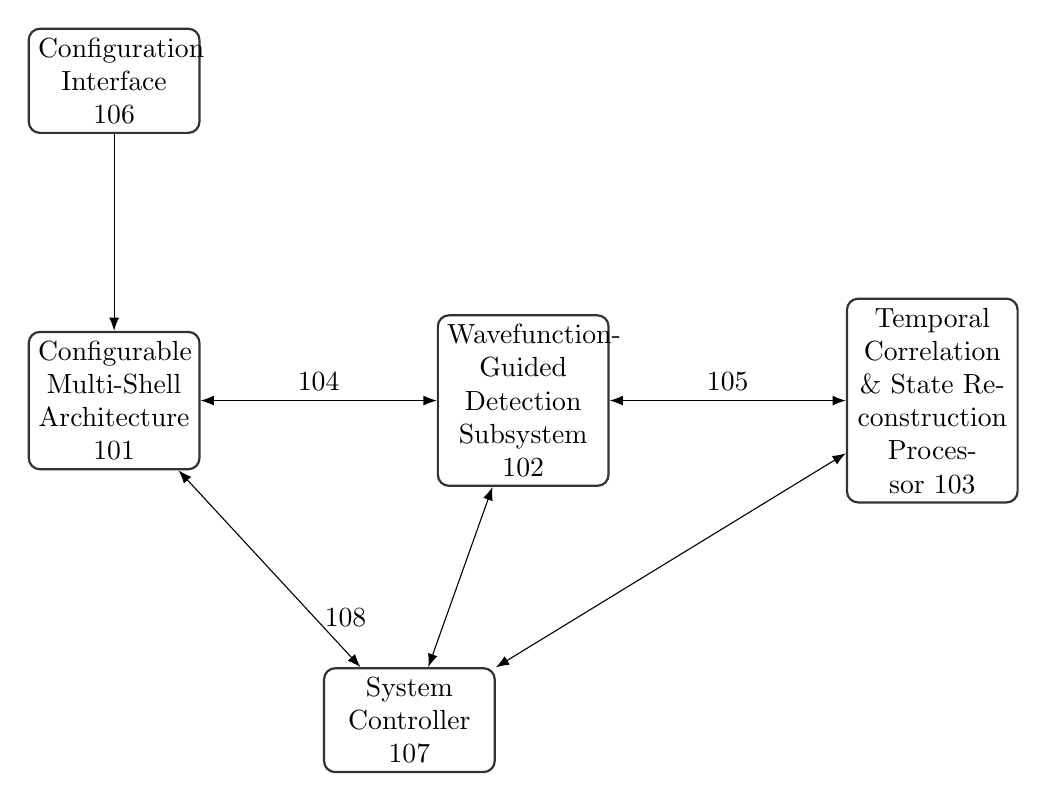
\begin{tikzpicture}[
    node distance=2.5cm and 3cm,
    block/.style={rectangle, draw, fill=white, text width=5.5em, text centered, rounded corners, minimum height=3em},
    mainblock/.style={rectangle, draw, fill=white, text width=5.5em, text centered, rounded corners, minimum height=3em, thick, draw=black!80},
    line/.style={draw, -Latex},
    bidirectional/.style={draw, Latex-Latex},
    scale=1.0
    ]
    
    % Define nodes
    \node[mainblock] (multiShell) {Configurable Multi-Shell Architecture 101};
    \node[mainblock, right=of multiShell] (detector) {Wavefunction-Guided Detection Subsystem 102};
    \node[mainblock, right=of detector] (processor) {Temporal Correlation \& State Reconstruction Processor 103};
    \node[mainblock, above=of multiShell] (interface) {Configuration Interface 106};
    \node[mainblock, below=of multiShell, xshift=3.75cm] (controller) {System Controller 107};
    
    % Define connections
    \draw[bidirectional] (multiShell) -- (detector) node[midway, above] {104};
    \draw[bidirectional] (detector) -- (processor) node[midway, above] {105};
    \draw[line] (interface) -- (multiShell);
    \draw[bidirectional] (controller) -- (multiShell) node[pos=0.25, right] {108};
    \draw[bidirectional] (controller) -- (detector);
    \draw[bidirectional] (controller) -- (processor);
    
\end{tikzpicture}
\caption*{FIG. 1}
\end{figure}

\begin{figure}[h]
\centering
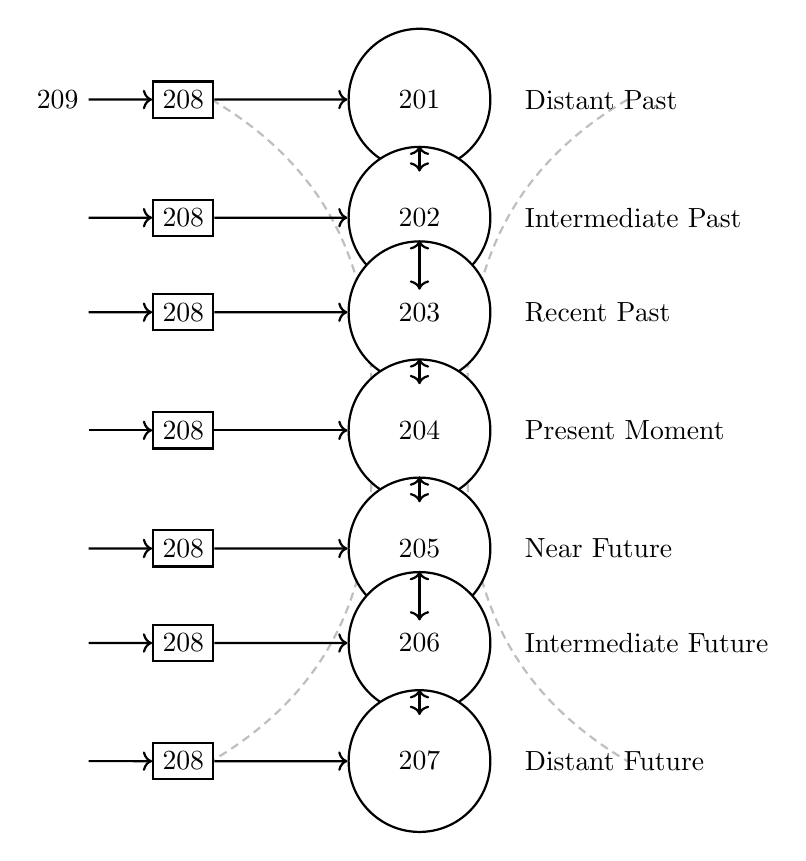
\begin{tikzpicture}[
    scale=1.2,
    shell/.style={circle, draw, thick, minimum size=1.8cm, fill=white},
    control/.style={rectangle, draw, thick, minimum width=0.5cm, minimum height=0.2cm, fill=white},
    connector/.style={thick, ->},
    line/.style={thick}
    ]
    
    % Define shells positions according to hourglass form
    \coordinate (center) at (0,0);
    
    % Draw the hourglass shape as a background
    \draw[thick, densely dashed, gray!50] 
        (-2.2,3.5) .. controls (-0.5,2.5) and (-0.5,1) .. (-0.5,0)
        .. controls (-0.5,-1) and (-0.5,-2.5) .. (-2.2,-3.5);
    
    \draw[thick, densely dashed, gray!50] 
        (2.2,3.5) .. controls (0.5,2.5) and (0.5,1) .. (0.5,0)
        .. controls (0.5,-1) and (0.5,-2.5) .. (2.2,-3.5);
    
    % Create shells
    \node[shell] (shell1) at (0,3.5) {201};
    \node[shell] (shell2) at (0,2.25) {202};
    \node[shell] (shell3) at (0,1.25) {203};
    \node[shell] (shell4) at (0,0) {204};
    \node[shell] (shell5) at (0,-1.25) {205};
    \node[shell] (shell6) at (0,-2.25) {206};
    \node[shell] (shell7) at (0,-3.5) {207};
    
    % Labels for temporal domains
    \node[right=0.3cm of shell1] {Distant Past};
    \node[right=0.3cm of shell2] {Intermediate Past};
    \node[right=0.3cm of shell3] {Recent Past};
    \node[right=0.3cm of shell4] {Present Moment};
    \node[right=0.3cm of shell5] {Near Future};
    \node[right=0.3cm of shell6] {Intermediate Future};
    \node[right=0.3cm of shell7] {Distant Future};
    
    % Control interfaces for each shell
    \node[control] (control1) at (-2.5,3.5) {208};
    \node[control] (control2) at (-2.5,2.25) {208};
    \node[control] (control3) at (-2.5,1.25) {208};
    \node[control] (control4) at (-2.5,0) {208};
    \node[control] (control5) at (-2.5,-1.25) {208};
    \node[control] (control6) at (-2.5,-2.25) {208};
    \node[control] (control7) at (-2.5,-3.5) {208};
    
    % Connect controls to shells
    \draw[connector] (control1) -- (shell1);
    \draw[connector] (control2) -- (shell2);
    \draw[connector] (control3) -- (shell3);
    \draw[connector] (control4) -- (shell4);
    \draw[connector] (control5) -- (shell5);
    \draw[connector] (control6) -- (shell6);
    \draw[connector] (control7) -- (shell7);
    
    % Control lines going off to the left
    \draw[line, <-] (control1) -- ++(-1,0) node[left] {209};
    \draw[line, <-] (control2) -- ++(-1,0);
    \draw[line, <-] (control3) -- ++(-1,0);
    \draw[line, <-] (control4) -- ++(-1,0);
    \draw[line, <-] (control5) -- ++(-1,0);
    \draw[line, <-] (control6) -- ++(-1,0);
    \draw[line, <-] (control7) -- ++(-1,0);
    
    % Coupling between shells
    \draw[line, <->] (shell1) -- (shell2);
    \draw[line, <->] (shell2) -- (shell3);
    \draw[line, <->] (shell3) -- (shell4);
    \draw[line, <->] (shell4) -- (shell5);
    \draw[line, <->] (shell5) -- (shell6);
    \draw[line, <->] (shell6) -- (shell7);
    
\end{tikzpicture}
\caption*{FIG. 2}
\end{figure}

\begin{figure}[h]
\centering
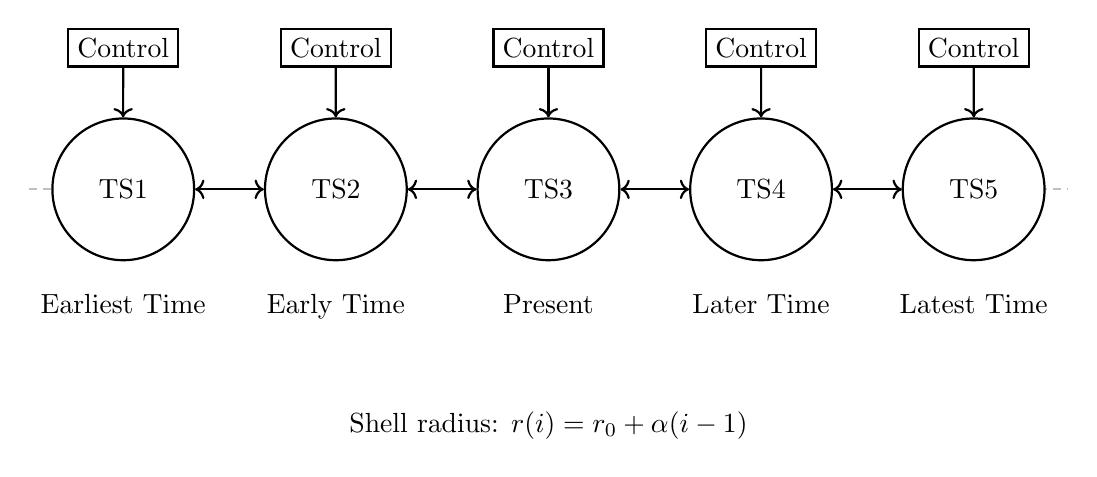
\begin{tikzpicture}[
    scale=1.2,
    shell/.style={circle, draw, thick, minimum size=1.8cm, fill=white},
    control/.style={rectangle, draw, thick, minimum width=0.5cm, minimum height=0.2cm, fill=white},
    connector/.style={thick, ->},
    line/.style={thick}
    ]
    
    % Define shells positions in linear form
    \coordinate (center) at (0,0);
    
    % Linear arrangement background line
    \draw[thick, densely dashed, gray!50] (-5.5,0) -- (5.5,0);
    
    % Create shells
    \node[shell] (shell1) at (-4.5,0) {TS1};
    \node[shell] (shell2) at (-2.25,0) {TS2};
    \node[shell] (shell3) at (0,0) {TS3};
    \node[shell] (shell4) at (2.25,0) {TS4};
    \node[shell] (shell5) at (4.5,0) {TS5};
    
    % Labels for temporal domains
    \node[below=0.3cm of shell1] {Earliest Time};
    \node[below=0.3cm of shell2] {Early Time};
    \node[below=0.3cm of shell3] {Present};
    \node[below=0.3cm of shell4] {Later Time};
    \node[below=0.3cm of shell5] {Latest Time};
    
    % Control interfaces for each shell
    \node[control] (control1) at (-4.5,1.5) {Control};
    \node[control] (control2) at (-2.25,1.5) {Control};
    \node[control] (control3) at (0,1.5) {Control};
    \node[control] (control4) at (2.25,1.5) {Control};
    \node[control] (control5) at (4.5,1.5) {Control};
    
    % Connect controls to shells
    \draw[connector] (control1) -- (shell1);
    \draw[connector] (control2) -- (shell2);
    \draw[connector] (control3) -- (shell3);
    \draw[connector] (control4) -- (shell4);
    \draw[connector] (control5) -- (shell5);
    
    % Coupling between shells
    \draw[line, <->] (shell1) -- (shell2);
    \draw[line, <->] (shell2) -- (shell3);
    \draw[line, <->] (shell3) -- (shell4);
    \draw[line, <->] (shell4) -- (shell5);
    
    % Mathematical formula for radius
    \node[align=center] at (0,-2.5) {Shell radius: $r(i) = r_0 + \alpha(i-1)$};
    
\end{tikzpicture}
\caption*{FIG. 3}
\end{figure}

\begin{figure}[h]
\centering
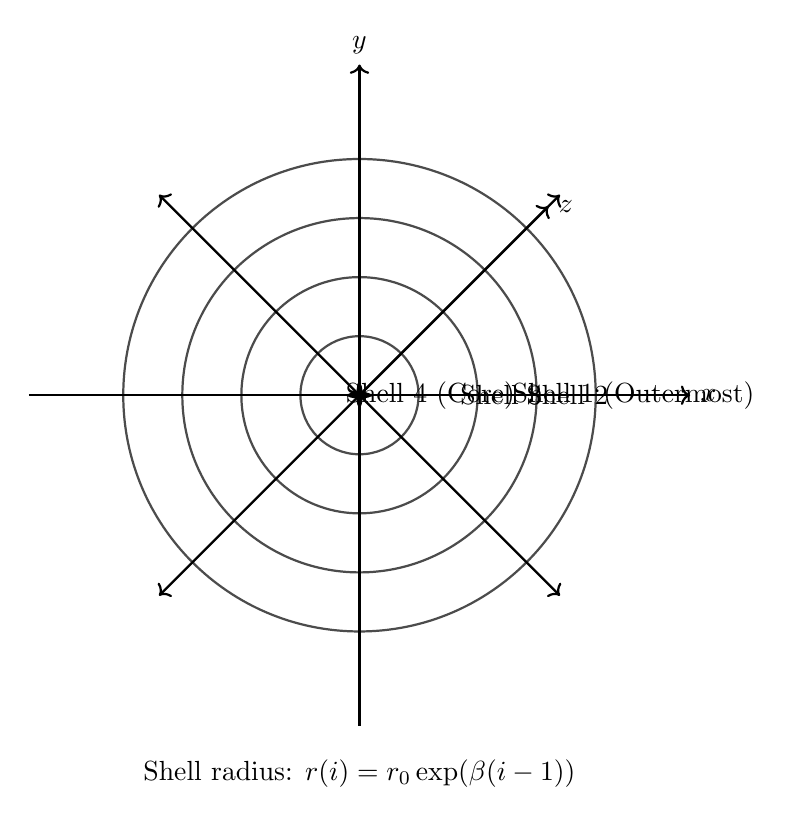
\begin{tikzpicture}[
    scale=1.2,
    shell/.style={circle, draw, thick, fill=white, opacity=0.7},
    line/.style={thick},
    connector/.style={thick, <->},
    ]
    
    % Create nested spherical shells
    \node[shell, minimum size=6cm] (shell1) at (0,0) {};
    \node[shell, minimum size=4.5cm] (shell2) at (0,0) {};
    \node[shell, minimum size=3cm] (shell3) at (0,0) {};
    \node[shell, minimum size=1.5cm] (shell4) at (0,0) {};
    
    % Label the shells
    \node at (2.9, 0) {Shell 1 (Outermost)};
    \node at (2.2, 0) {Shell 2};
    \node at (1.5, 0) {Shell 3};
    \node at (0.75, 0) {Shell 4 (Core)};
    
    % Draw radial connectors between shells
    \draw[connector] (0,0) -- (45:3);
    \draw[connector] (0,0) -- (135:3);
    \draw[connector] (0,0) -- (225:3);
    \draw[connector] (0,0) -- (315:3);
    
    % Add some coordinate axes
    \draw[->, thick] (-3.5,0) -- (3.5,0) node[right] {$x$};
    \draw[->, thick] (0,-3.5) -- (0,3.5) node[above] {$y$};
    \draw[->, thick] (0,0) -- (2,2) node[right] {$z$};
    
    % Mathematical formula for radius
    \node[align=center] at (0,-4) {Shell radius: $r(i) = r_0 \exp(\beta (i-1))$};
    
\end{tikzpicture}
\caption*{FIG. 4}
\end{figure}

\begin{figure}[h]
\centering
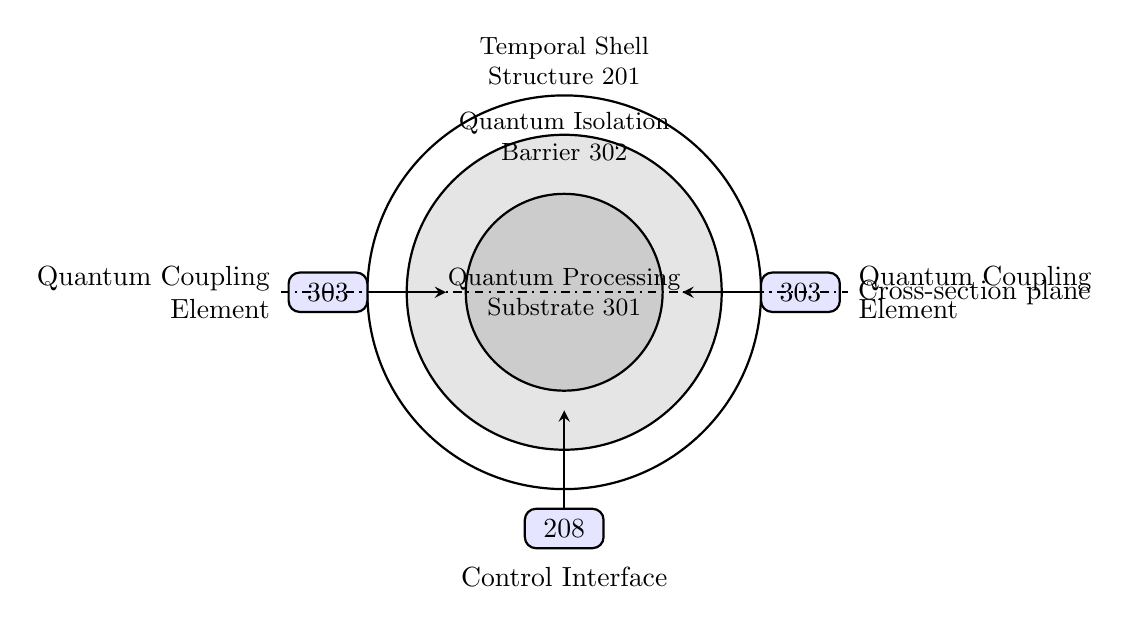
\begin{tikzpicture}[
    scale=1.2,
    outer/.style={circle, draw, thick, minimum size=5cm, fill=white},
    middle/.style={circle, draw, thick, minimum size=4cm, fill=gray!20},
    inner/.style={circle, draw, thick, minimum size=2.5cm, fill=gray!40},
    connector/.style={thick, ->, >=stealth},
    quantum/.style={draw, thick, fill=blue!10, rectangle, rounded corners, minimum width=1cm, minimum height=0.5cm},
    label/.style={font=\small}
    ]
    
    % Create main shell structure
    \node[outer] (shell) at (0,0) {};
    \node[middle] (barrier) at (0,0) {};
    \node[inner] (substrate) at (0,0) {};
    
    % Add labels
    \node[label, align=center] at (0,0) {Quantum Processing\\Substrate 301};
    \node[label, align=center] at (0,1.65) {Quantum Isolation\\Barrier 302};
    \node[label, align=center] at (0,2.45) {Temporal Shell\\Structure 201};
    
    % Add quantum coupling elements
    \node[quantum] (coupling1) at (2.5,0) {303};
    \node[quantum] (coupling2) at (-2.5,0) {303};
    \node[quantum] (control) at (0,-2.5) {208};
    
    % Draw connectors
    \draw[connector] (coupling1) -- (1.25,0);
    \draw[connector] (coupling2) -- (-1.25,0);
    \draw[connector] (control) -- (0,-1.25);
    
    % Add detailed labels
    \node[right=0.1cm of coupling1, align=left] {Quantum Coupling\\Element};
    \node[left=0.1cm of coupling2, align=right] {Quantum Coupling\\Element};
    \node[below=0.1cm of control, align=center] {Control Interface};
    
    % Cross-section indicator
    \draw[thick, dashdotted] (-3,0) -- (3,0) node[right] {Cross-section plane};
    
\end{tikzpicture}
\caption*{FIG. 5}
\end{figure}

\begin{figure}[h]
\centering
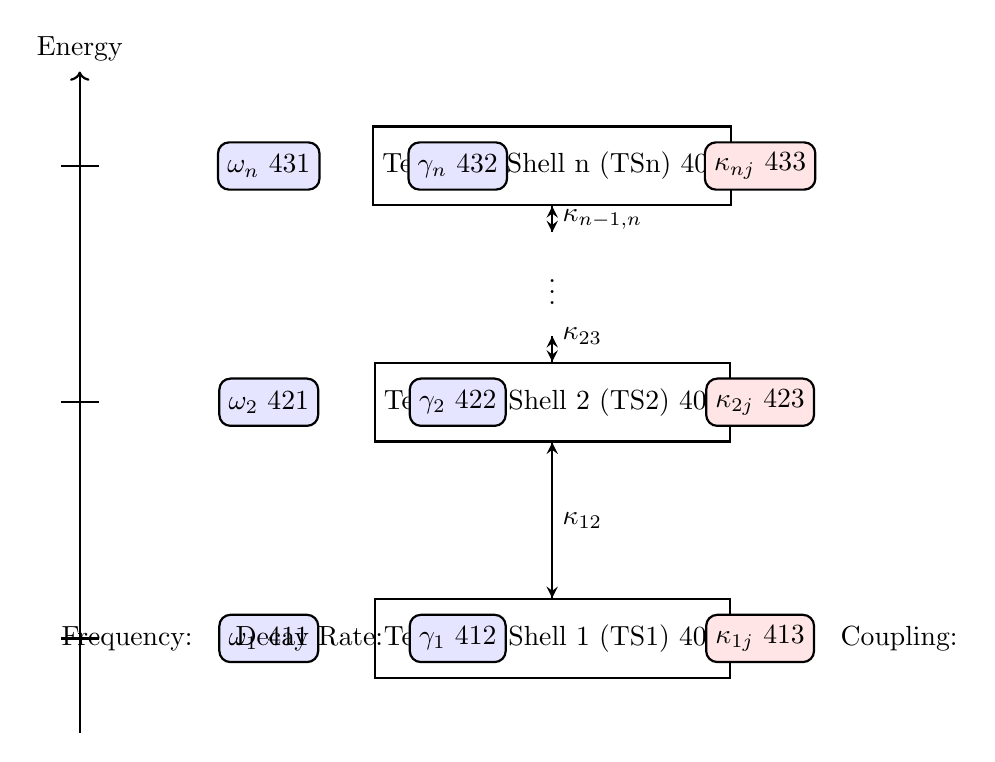
\begin{tikzpicture}[
    scale=1.2,
    shell/.style={rectangle, draw, thick, minimum height=1cm, minimum width=3.5cm, fill=white},
    param/.style={rectangle, draw, thick, minimum height=0.6cm, minimum width=1.2cm, fill=blue!10, rounded corners},
    coupling/.style={rectangle, draw, thick, minimum height=0.6cm, minimum width=1.2cm, fill=red!10, rounded corners},
    arrow/.style={->, >=stealth, thick},
    ]
    
    % Define shell positions
    \coordinate (ts1) at (0,0);
    \coordinate (ts2) at (0,2.5);
    \coordinate (tsn) at (0,5);
    
    % Create shells
    \node[shell] (shell1) at (ts1) {Temporal Shell 1 (TS1) 401};
    \node[shell] (shell2) at (ts2) {Temporal Shell 2 (TS2) 402};
    \node at (0,3.75) {\vdots};
    \node[shell] (shelln) at (tsn) {Temporal Shell n (TSn) 403};
    
    % Add parameters for shell 1
    \node[param] (freq1) at (-3,0) {$\omega_1$ 411};
    \node[param] (decay1) at (-1,0) {$\gamma_1$ 412};
    \node[coupling] (coupling1) at (2.2,0) {$\kappa_{1j}$ 413};
    
    % Add parameters for shell 2
    \node[param] (freq2) at (-3,2.5) {$\omega_2$ 421};
    \node[param] (decay2) at (-1,2.5) {$\gamma_2$ 422};
    \node[coupling] (coupling2) at (2.2,2.5) {$\kappa_{2j}$ 423};
    
    % Add parameters for shell n
    \node[param] (freqn) at (-3,5) {$\omega_n$ 431};
    \node[param] (decayn) at (-1,5) {$\gamma_n$ 432};
    \node[coupling] (couplingn) at (2.2,5) {$\kappa_{nj}$ 433};
    
    % Create parameter labels
    \node[left=0.2cm of freq1] {Frequency:};
    \node[left=0.2cm of decay1] {Decay Rate:};
    \node[right=0.2cm of coupling1] {Coupling:};
    
    % Connect shells with coupling arrows
    \draw[arrow] (shell1.north) -- (shell2.south) node[midway, right] {$\kappa_{12}$};
    \draw[arrow] (shell2.south) -- (shell1.north);
    \draw[arrow] (shell2.north) -- (0,3.2) node[right] {$\kappa_{23}$};
    \draw[arrow] (0,3.2) -- (shell2.north);
    \draw[arrow] (0,4.3) -- (shelln.south) node[midway, right] {$\kappa_{n-1,n}$};
    \draw[arrow] (shelln.south) -- (0,4.3);
    
    % Energy scale
    \draw[thick, ->] (-5,-1) -- (-5,6) node[above] {Energy};
    \foreach \y in {0,2.5,5} {
        \draw[thick] (-5.2,\y) -- (-4.8,\y);
    }
    
\end{tikzpicture}
\caption*{FIG. 6}
\end{figure}

\begin{figure}[h]
\centering
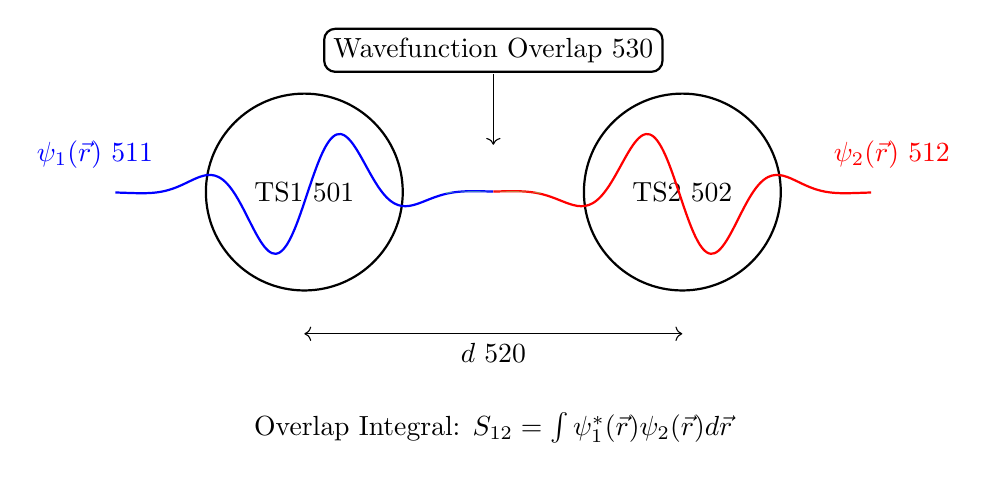
\begin{tikzpicture}[
    scale=1.2,
    shell/.style={circle, draw, thick, minimum size=2.5cm, fill=white},
    wave/.style={thick, smooth},
    fill_wave/.style={smooth, fill=blue!20, opacity=0.5},
    ]
    
    % Define shell positions
    \coordinate (ts1center) at (-2,0);
    \coordinate (ts2center) at (2,0);
    
    % Draw shells
    \node[shell] (ts1) at (ts1center) {TS1 501};
    \node[shell] (ts2) at (ts2center) {TS2 502};
    
    % Add separation distance label
    \draw[<->] (-2,-1.5) -- (2,-1.5) node[midway, below] {$d$ 520};
    
    % Draw wavefunction for TS1
    \draw[wave, blue] plot[domain=-4:0, samples=100] 
        (\x, {exp(-(\x+2)*(\x+2)/0.8)*cos(4*\x r)*0.75});
    \node[blue, left] at (-3.5,0.4) {$\psi_1(\vec{r})$ 511};
    
    % Draw wavefunction for TS2
    \draw[wave, red] plot[domain=0:4, samples=100] 
        (\x, {exp(-(\x-2)*(\x-2)/0.8)*cos(4*\x r)*0.75});
    \node[red, right] at (3.5,0.4) {$\psi_2(\vec{r})$ 512};
    
    % Fill the overlap region
    \fill[fill_wave, green!50] plot[domain=-0.5:0.5, samples=100] 
        (\x, {exp(-(\x+2)*(\x+2)/0.8)*cos(4*\x r)*0.75}) -- 
        plot[domain=0.5:-0.5, samples=100] 
        (\x, {exp(-(\x-2)*(\x-2)/0.8)*cos(4*\x r)*0.75});
    
    % Label the overlap region
    \node[draw, thick, fill=white, rounded corners] at (0,1.5) {Wavefunction Overlap 530};
    \draw[->] (0,1.25) -- (0,0.5);
    
    % Add mathematical equation for overlap integral
    \node[align=center] at (0,-2.5) {Overlap Integral: $S_{12} = \int \psi_1^*(\vec{r})\psi_2(\vec{r})d\vec{r}$};
    
\end{tikzpicture}
\caption*{FIG. 7}
\end{figure}

\begin{figure}[h]
\centering
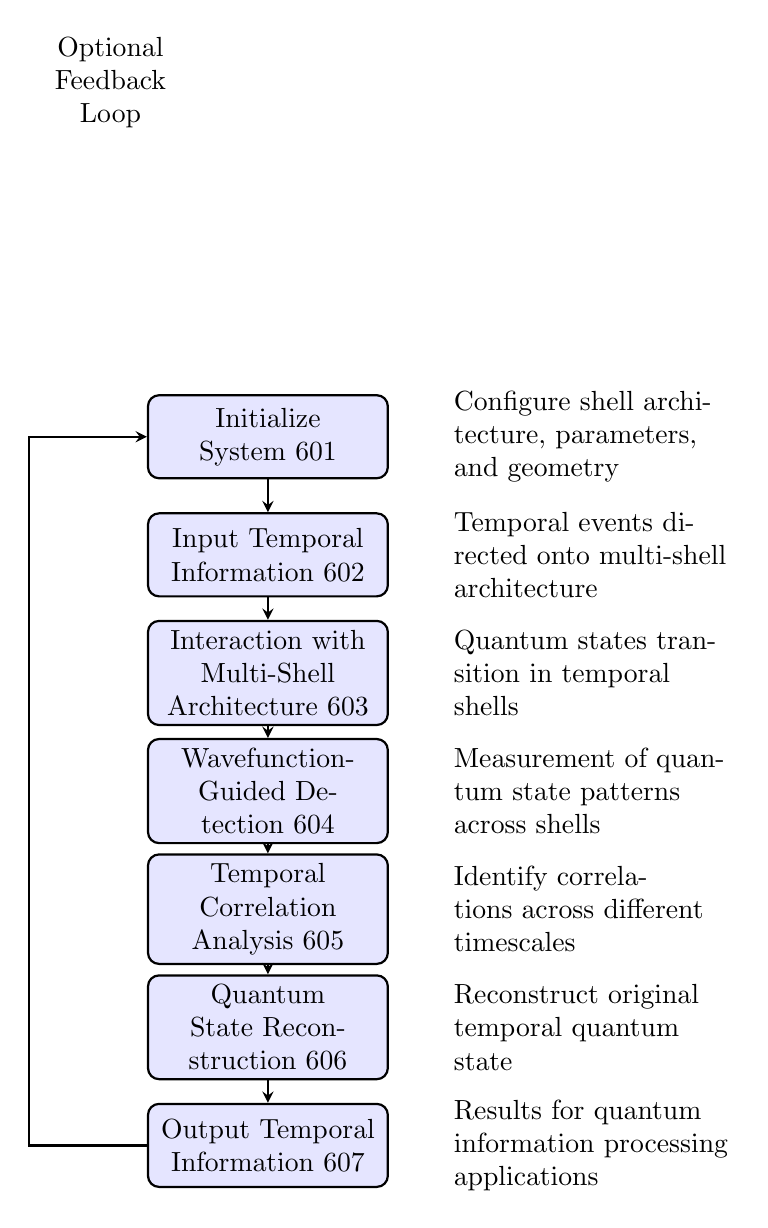
\begin{tikzpicture}[
    scale=1.0,
    block/.style={rectangle, draw, thick, fill=blue!10, text width=8em, text centered, rounded corners, minimum height=3em},
    line/.style={draw, ->, >=stealth, thick},
    ]
    
    % Define block positions
    \node[block] (init) at (0,0) {Initialize System 601};
    \node[block] (input) at (0,-1.5) {Input Temporal Information 602};
    \node[block] (interact) at (0,-3) {Interaction with Multi-Shell Architecture 603};
    \node[block] (detect) at (0,-4.5) {Wavefunction-Guided Detection 604};
    \node[block] (process) at (0,-6) {Temporal Correlation Analysis 605};
    \node[block] (reconstruct) at (0,-7.5) {Quantum State Reconstruction 606};
    \node[block] (output) at (0,-9) {Output Temporal Information 607};
    
    % Connect blocks with arrows
    \draw[line] (init) -- (input);
    \draw[line] (input) -- (interact);
    \draw[line] (interact) -- (detect);
    \draw[line] (detect) -- (process);
    \draw[line] (process) -- (reconstruct);
    \draw[line] (reconstruct) -- (output);
    
    % Add detail annotations
    \node[right=0.7cm of init, text width=10em, align=left] {Configure shell architecture, parameters, and geometry};
    \node[right=0.7cm of input, text width=10em, align=left] {Temporal events directed onto multi-shell architecture};
    \node[right=0.7cm of interact, text width=10em, align=left] {Quantum states transition in temporal shells};
    \node[right=0.7cm of detect, text width=10em, align=left] {Measurement of quantum state patterns across shells};
    \node[right=0.7cm of process, text width=10em, align=left] {Identify correlations across different timescales};
    \node[right=0.7cm of reconstruct, text width=10em, align=left] {Reconstruct original temporal quantum state};
    \node[right=0.7cm of output, text width=10em, align=left] {Results for quantum information processing applications};
    
    % Add a feedback loop
    \draw[line] (output.west) -- ++(-1.5,0) -- ++(0,9) -- (init.west);
    \node[text width=5em, align=center] at (-2,4.5) {Optional\\Feedback\\Loop};
    
\end{tikzpicture}
\caption*{FIG. 8}
\end{figure}

\begin{figure}[h]
\centering
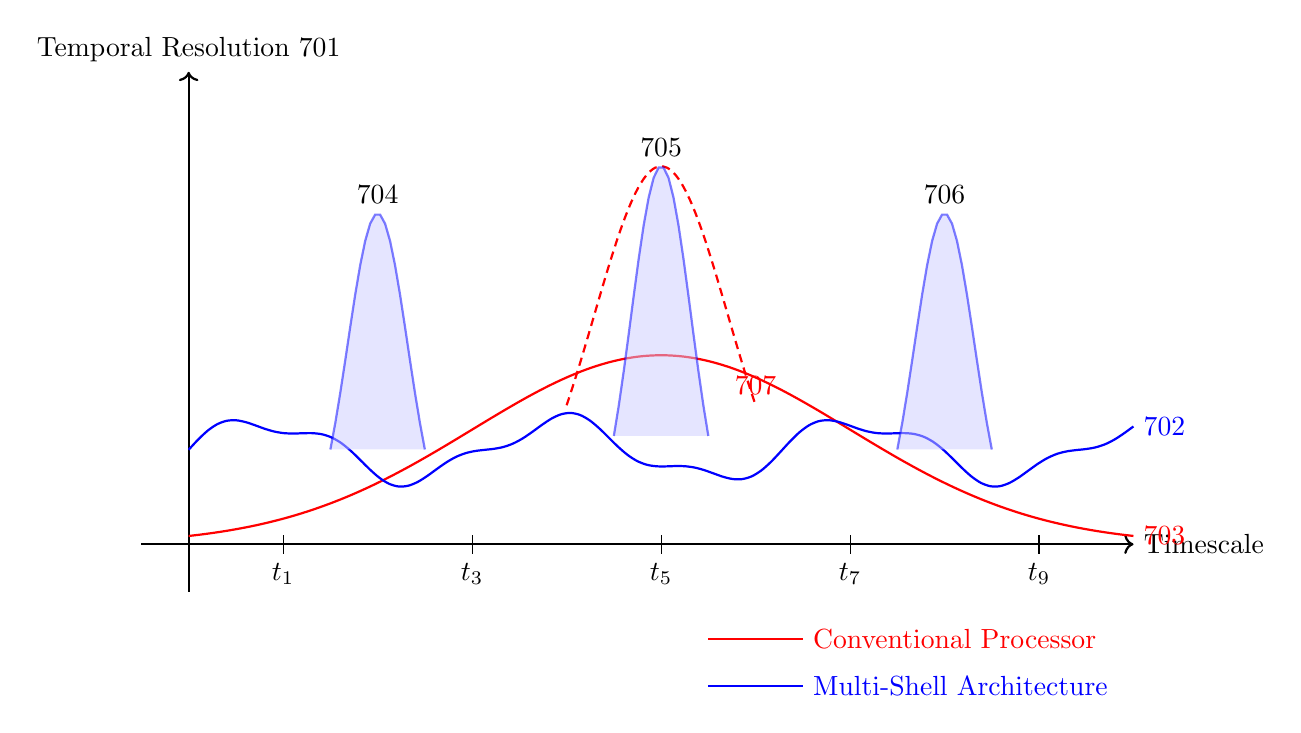
\begin{tikzpicture}[
    scale=1.2,
    axis/.style={thick, ->},
    conventional/.style={thick, red, smooth},
    multishell/.style={thick, blue, smooth},
    peak/.style={blue, thick, fill=blue!20, opacity=0.5},
    ]
    
    % Set up axes
    \draw[axis] (-0.5,0) -- (10,0) node[right] {Timescale};
    \draw[axis] (0,-0.5) -- (0,5) node[above] {Temporal Resolution 701};
    
    % Add axis labels
    \foreach \x in {1,3,5,7,9} {
        \draw (\x,-0.1) -- (\x,0.1);
        \node[below] at (\x,-0.1) {$t_{\x}$};
    }
    
    % Draw conventional system response curve
    \draw[conventional] plot[domain=0:10, samples=100] 
        (\x, {2*exp(-(\x-5)*(\x-5)/8)}) node[right] {703};
    
    % Draw the narrower conventional peak
    \draw[conventional, densely dashed] plot[domain=4:6, samples=50] 
        (\x, {4*exp(-(\x-5)*(\x-5)/1)}) node[above] {707};
    
    % Draw multi-shell system response curve
    \draw[multishell] plot[domain=0:10, samples=100] 
        (\x, {1 + 0.3*sin(2*\x r) + 0.1*sin(5*\x r)}) node[right] {702};
    
    % Add resolution peaks
    \draw[peak] plot[domain=1.5:2.5, samples=20] 
        (\x, {3.5*exp(-(\x-2)*(\x-2)/0.2)});
    \node at (2,3.7) {704};
    
    \draw[peak] plot[domain=4.5:5.5, samples=20] 
        (\x, {4*exp(-(\x-5)*(\x-5)/0.2)});
    \node at (5,4.2) {705};
    
    \draw[peak] plot[domain=7.5:8.5, samples=20] 
        (\x, {3.5*exp(-(\x-8)*(\x-8)/0.2)});
    \node at (8,3.7) {706};
    
    % Add legend
    \draw[conventional] (5.5,-1) -- (6.5,-1) node[right] {Conventional Processor};
    \draw[multishell] (5.5,-1.5) -- (6.5,-1.5) node[right] {Multi-Shell Architecture};
    
\end{tikzpicture}
\caption*{FIG. 9}
\end{figure}

\begin{figure}[h]
\centering
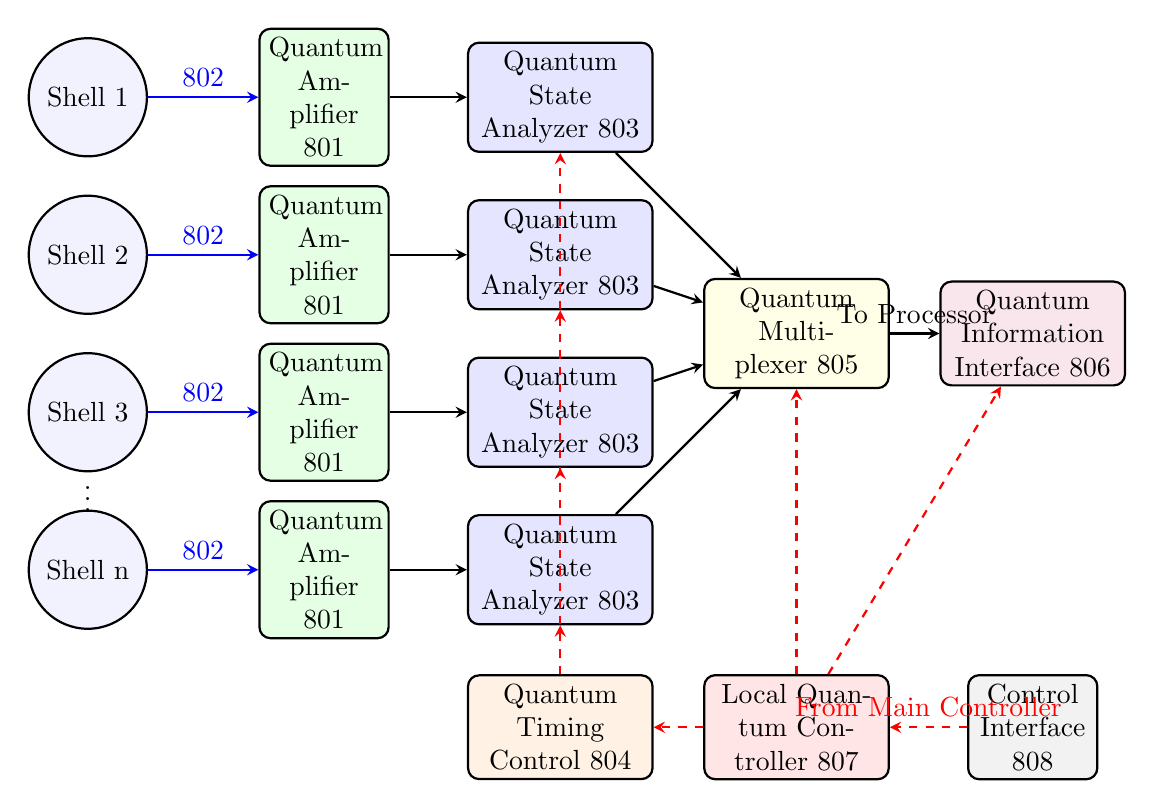
\begin{tikzpicture}[
    scale=1.0,
    block/.style={rectangle, draw, thick, fill=blue!10, text width=6em, text centered, rounded corners, minimum height=2.5em},
    smallblock/.style={rectangle, draw, thick, fill=green!10, text width=4em, text centered, rounded corners, minimum height=2em},
    shell/.style={circle, draw, thick, minimum size=1.5cm, fill=blue!5},
    quantum/.style={thick, ->, >=stealth, blue},
    control/.style={thick, ->, >=stealth, red, dashed},
    data/.style={thick, ->, >=stealth},
    ]
    
    % Place shells
    \node[shell] (shell1) at (-6,3) {Shell 1};
    \node[shell] (shell2) at (-6,1) {Shell 2};
    \node[shell] (shell3) at (-6,-1) {Shell 3};
    \node at (-6,-2) {\vdots};
    \node[shell] (shelln) at (-6,-3) {Shell n};
    
    % Place quantum amplifiers
    \node[smallblock] (amp1) at (-3,3) {Quantum Amplifier 801};
    \node[smallblock] (amp2) at (-3,1) {Quantum Amplifier 801};
    \node[smallblock] (amp3) at (-3,-1) {Quantum Amplifier 801};
    \node[smallblock] (ampn) at (-3,-3) {Quantum Amplifier 801};
    
    % Place quantum state analyzers
    \node[block] (analyzer1) at (0,3) {Quantum State Analyzer 803};
    \node[block] (analyzer2) at (0,1) {Quantum State Analyzer 803};
    \node[block] (analyzer3) at (0,-1) {Quantum State Analyzer 803};
    \node[block] (analyzern) at (0,-3) {Quantum State Analyzer 803};
    
    % Place quantum multiplexer
    \node[block, fill=yellow!10] (mux) at (3,0) {Quantum Multiplexer 805};
    
    % Place quantum interface
    \node[block, fill=purple!10] (interface) at (6,0) {Quantum Information Interface 806};
    
    % Place timing control
    \node[block, fill=orange!10] (timing) at (0,-5) {Quantum Timing Control 804};
    
    % Place controller
    \node[block, fill=red!10] (controller) at (3,-5) {Local Quantum Controller 807};
    
    % Place main controller interface
    \node[smallblock, fill=gray!10] (controlInterface) at (6,-5) {Control Interface 808};
    
    % Connect shells to amplifiers with quantum channels
    \draw[quantum] (shell1) -- (amp1) node[midway, above] {802};
    \draw[quantum] (shell2) -- (amp2) node[midway, above] {802};
    \draw[quantum] (shell3) -- (amp3) node[midway, above] {802};
    \draw[quantum] (shelln) -- (ampn) node[midway, above] {802};
    
    % Connect amplifiers to analyzers
    \draw[data] (amp1) -- (analyzer1);
    \draw[data] (amp2) -- (analyzer2);
    \draw[data] (amp3) -- (analyzer3);
    \draw[data] (ampn) -- (analyzern);
    
    % Connect analyzers to multiplexer
    \draw[data] (analyzer1) -- (mux);
    \draw[data] (analyzer2) -- (mux);
    \draw[data] (analyzer3) -- (mux);
    \draw[data] (analyzern) -- (mux);
    
    % Connect multiplexer to interface
    \draw[data] (mux) -- (interface) node[midway, above] {To Processor};
    
    % Connect timing control to analyzers
    \draw[control] (timing) -- (analyzer1);
    \draw[control] (timing) -- (analyzer2);
    \draw[control] (timing) -- (analyzer3);
    \draw[control] (timing) -- (analyzern);
    
    % Connect controller
    \draw[control] (controller) -- (timing);
    \draw[control] (controller) -- (mux);
    \draw[control] (controller) -- (interface);
    
    % Connect main controller interface
    \draw[control] (controlInterface) -- (controller) node[midway, above] {From Main Controller};
    
\end{tikzpicture}
\caption*{FIG. 10}
\end{figure}

\end{document}
